% -----------------------
\subsection{Pfeilspitzen}
% -----------------------
\begin{minipage}{0.7\textwidth}
  \footnotesize
  % parcolor version 2011-09-30
\begingroup
\ttfamily
\definecolor{R}{named}{Red}
\definecolor{G}{named}{ForestGreen}
\definecolor{B}{named}{RoyalBlue}
\definecolor{C}{named}{Cyan}
\definecolor{M}{named}{Magenta}
\definecolor{Y}{named}{YellowOrange}
\definecolor{background}{rgb}{0.82, 0.82, 0.92}
\dimen255=\textwidth
\advance\dimen255 by -2\fboxsep
\noindent
\colorbox{background}
{%
\parbox{\dimen255}
{%
\rule[-0.5ex]{0pt}{2.5ex}\hspace*{0.0em}\textbackslash{}draw[\textcolor{R}{\textbf{{-}{>}}}]~(0,~0)~{-}{-}~(3,~0);}%
}%
\endgroup

\end{minipage}\hfill
\begin{minipage}{0.29\textwidth}
  \centering
  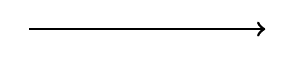
\begin{tikzpicture}[line width=1pt]
    % Pfeilspitze rechts
    \draw[->] (0, 0) -- (3, 0);
  \end{tikzpicture}
\end{minipage}

\begin{minipage}{0.7\textwidth}
  \footnotesize
  % parcolor version 2011-09-30
\begingroup
\ttfamily
\definecolor{R}{named}{Red}
\definecolor{G}{named}{ForestGreen}
\definecolor{B}{named}{RoyalBlue}
\definecolor{C}{named}{Cyan}
\definecolor{M}{named}{Magenta}
\definecolor{Y}{named}{YellowOrange}
\definecolor{background}{rgb}{0.82, 0.82, 0.92}
\dimen255=\textwidth
\advance\dimen255 by -2\fboxsep
\noindent
\colorbox{background}
{%
\parbox{\dimen255}
{%
\rule[-0.5ex]{0pt}{2.5ex}\hspace*{0.0em}\textbackslash{}draw[\textcolor{R}{\textbf{{<}{-}}}]~(0,~0)~{-}{-}~(3,~0);}%
}%
\endgroup

\end{minipage}\hfill
\begin{minipage}{0.29\textwidth}
  \centering
  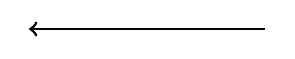
\begin{tikzpicture}[line width=1pt]
    % Pfeilspitze links
    \draw[<-] (0, 0) -- (3, 0);
  \end{tikzpicture}
\end{minipage}

\begin{minipage}{0.7\textwidth}
  \footnotesize
  % parcolor version 2011-09-30
\begingroup
\ttfamily
\definecolor{R}{named}{Red}
\definecolor{G}{named}{ForestGreen}
\definecolor{B}{named}{RoyalBlue}
\definecolor{C}{named}{Cyan}
\definecolor{M}{named}{Magenta}
\definecolor{Y}{named}{YellowOrange}
\definecolor{background}{rgb}{0.82, 0.82, 0.92}
\dimen255=\textwidth
\advance\dimen255 by -2\fboxsep
\noindent
\colorbox{background}
{%
\parbox{\dimen255}
{%
\rule[-0.5ex]{0pt}{2.5ex}\hspace*{0.0em}\textbackslash{}draw[\textcolor{R}{\textbf{{<}{-}{>}}}]~(0,~0)~{-}{-}~(3,~0);}%
}%
\endgroup

\end{minipage}\hfill
\begin{minipage}{0.29\textwidth}
  \centering
  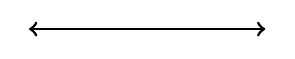
\begin{tikzpicture}[line width=1pt]
    % Pfeilspitzen links und rechts
    \draw[<->] (0, 0) -- (3, 0);
  \end{tikzpicture}
\end{minipage}

\begin{minipage}{0.7\textwidth}
  \footnotesize
  % parcolor version 2011-09-30
\begingroup
\ttfamily
\definecolor{R}{named}{Red}
\definecolor{G}{named}{ForestGreen}
\definecolor{B}{named}{RoyalBlue}
\definecolor{C}{named}{Cyan}
\definecolor{M}{named}{Magenta}
\definecolor{Y}{named}{YellowOrange}
\definecolor{background}{rgb}{0.82, 0.82, 0.92}
\dimen255=\textwidth
\advance\dimen255 by -2\fboxsep
\noindent
\colorbox{background}
{%
\parbox{\dimen255}
{%
\rule[-0.5ex]{0pt}{2.5ex}\hspace*{0.0em}\textbackslash{}draw[\textcolor{R}{\textbf{{<}{<}{-}{>}{>}}}]~(0,~0)~{-}{-}~(3,~0);}%
}%
\endgroup

\end{minipage}\hfill
\begin{minipage}{0.29\textwidth}
  \centering
  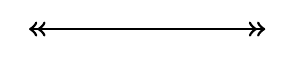
\begin{tikzpicture}[line width=1pt]
    % doppelte Spitze
    \draw[<<->>] (0, 0) -- (3, 0);
  \end{tikzpicture}
\end{minipage}

\begin{minipage}{0.7\textwidth}
  \footnotesize
  % parcolor version 2011-09-30
\begingroup
\ttfamily
\definecolor{R}{named}{Red}
\definecolor{G}{named}{ForestGreen}
\definecolor{B}{named}{RoyalBlue}
\definecolor{C}{named}{Cyan}
\definecolor{M}{named}{Magenta}
\definecolor{Y}{named}{YellowOrange}
\definecolor{background}{rgb}{0.82, 0.82, 0.92}
\dimen255=\textwidth
\advance\dimen255 by -2\fboxsep
\noindent
\colorbox{background}
{%
\parbox{\dimen255}
{%
\rule[-0.5ex]{0pt}{2.5ex}\hspace*{0.0em}\textbackslash{}draw[\textcolor{R}{\textbf{|{-}|}}]~(0,~0)~{-}{-}~(3,~0);}%
}%
\endgroup

\end{minipage}\hfill
\begin{minipage}{0.29\textwidth}
  \centering
  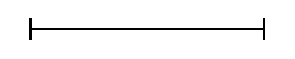
\begin{tikzpicture}[line width=1pt]
    % stumpfe Enden
    \draw[|-|] (0, 0) -- (3, 0);
  \end{tikzpicture}
\end{minipage}

\begin{minipage}{0.7\textwidth}
  \footnotesize
  % parcolor version 2011-09-30
\begingroup
\ttfamily
\definecolor{R}{named}{Red}
\definecolor{G}{named}{ForestGreen}
\definecolor{B}{named}{RoyalBlue}
\definecolor{C}{named}{Cyan}
\definecolor{M}{named}{Magenta}
\definecolor{Y}{named}{YellowOrange}
\definecolor{background}{rgb}{0.82, 0.82, 0.92}
\dimen255=\textwidth
\advance\dimen255 by -2\fboxsep
\noindent
\colorbox{background}
{%
\parbox{\dimen255}
{%
\rule[-0.5ex]{0pt}{2.5ex}\hspace*{0.0em}\textbackslash{}draw[\textcolor{R}{\textbf{|{<}{-}{>}|}},~\textcolor{R}{\textbf{{>}=latex}}]~(0,~0)~{-}{-}~(3,~0);}%
}%
\endgroup

\end{minipage}\hfill
\begin{minipage}{0.29\textwidth}
  \centering
  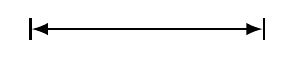
\begin{tikzpicture}[line width=1pt]
    % Spitze mit Begrenzung
    \draw[|<->|, >=latex] (0, 0) -- (3, 0);
  \end{tikzpicture}
\end{minipage}

\begin{minipage}{0.7\textwidth}
  \footnotesize
  % parcolor version 2011-09-30
\begingroup
\ttfamily
\definecolor{R}{named}{Red}
\definecolor{G}{named}{ForestGreen}
\definecolor{B}{named}{RoyalBlue}
\definecolor{C}{named}{Cyan}
\definecolor{M}{named}{Magenta}
\definecolor{Y}{named}{YellowOrange}
\definecolor{background}{rgb}{0.82, 0.82, 0.92}
\dimen255=\textwidth
\advance\dimen255 by -2\fboxsep
\noindent
\colorbox{background}
{%
\parbox{\dimen255}
{%
\rule[-0.5ex]{0pt}{2.5ex}\hspace*{0.0em}\textbackslash{}draw[{<}{-}{>},~\textcolor{R}{\textbf{{>}=latex}}]~(0,~0)~{-}{-}~(3,~0);}%
}%
\endgroup

\end{minipage}\hfill
\begin{minipage}{0.29\textwidth}
  \centering
  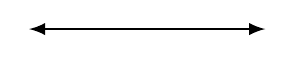
\begin{tikzpicture}[line width=1pt]
    % Form: latex
    \draw[<->, >=latex] (0, 0) -- (3, 0);
  \end{tikzpicture}
\end{minipage}

\begin{minipage}{0.7\textwidth}
  \footnotesize
  % parcolor version 2011-09-30
\begingroup
\ttfamily
\definecolor{R}{named}{Red}
\definecolor{G}{named}{ForestGreen}
\definecolor{B}{named}{RoyalBlue}
\definecolor{C}{named}{Cyan}
\definecolor{M}{named}{Magenta}
\definecolor{Y}{named}{YellowOrange}
\definecolor{background}{rgb}{0.82, 0.82, 0.92}
\dimen255=\textwidth
\advance\dimen255 by -2\fboxsep
\noindent
\colorbox{background}
{%
\parbox{\dimen255}
{%
\rule[-0.5ex]{0pt}{2.5ex}\hspace*{0.0em}\textbackslash{}draw[{<}{-}{>},~\textcolor{R}{\textbf{{>}=stealth}}]~(0,~0)~{-}{-}~(3,~0);}%
}%
\endgroup

\end{minipage}\hfill
\begin{minipage}{0.29\textwidth}
  \centering
  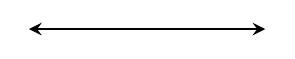
\begin{tikzpicture}[line width=1pt]
    % Form: stealth
    \draw[<->, >=stealth] (0, 0) -- (3, 0);
  \end{tikzpicture}
\end{minipage}

\begin{minipage}{0.7\textwidth}
  \footnotesize
  % parcolor version 2011-09-30
\begingroup
\ttfamily
\definecolor{R}{named}{Red}
\definecolor{G}{named}{ForestGreen}
\definecolor{B}{named}{RoyalBlue}
\definecolor{C}{named}{Cyan}
\definecolor{M}{named}{Magenta}
\definecolor{Y}{named}{YellowOrange}
\definecolor{background}{rgb}{0.82, 0.82, 0.92}
\dimen255=\textwidth
\advance\dimen255 by -2\fboxsep
\noindent
\colorbox{background}
{%
\parbox{\dimen255}
{%
\rule[-0.5ex]{0pt}{2.5ex}\hspace*{0.0em}\textbackslash{}draw[{<}{<}{-}{>}{>},~\textcolor{R}{\textbf{{>}=to~reversed}}]~(0,~0)~{-}{-}~(3,~0);}%
}%
\endgroup

\end{minipage}\hfill
\begin{minipage}{0.29\textwidth}
  \centering
  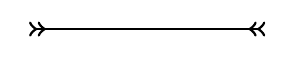
\begin{tikzpicture}[line width=1pt]
    % doppelte Spitze: to reversed
    \draw[<<->>, >=to reversed] (0, 0) -- (3, 0);
  \end{tikzpicture}
\end{minipage}

\begin{minipage}{0.7\textwidth}
  \footnotesize
  % parcolor version 2011-09-30
\begingroup
\ttfamily
\definecolor{R}{named}{Red}
\definecolor{G}{named}{ForestGreen}
\definecolor{B}{named}{RoyalBlue}
\definecolor{C}{named}{Cyan}
\definecolor{M}{named}{Magenta}
\definecolor{Y}{named}{YellowOrange}
\definecolor{background}{rgb}{0.82, 0.82, 0.92}
\dimen255=\textwidth
\advance\dimen255 by -2\fboxsep
\noindent
\colorbox{background}
{%
\parbox{\dimen255}
{%
\rule[-0.5ex]{0pt}{2.5ex}\hspace*{0.0em}\textbackslash{}draw[{<}{<}{-}{>}{>},~\textcolor{R}{\textbf{{>}=stealth~reversed}}]~(0,~0)~{-}{-}~(3,~0);}%
}%
\endgroup

\end{minipage}\hfill
\begin{minipage}{0.29\textwidth}
  \centering
  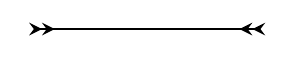
\begin{tikzpicture}[line width=1pt]
    % doppelte Spitze: stealth reversed
    \draw[<<->>, >=stealth reversed] (0, 0) -- (3, 0);
  \end{tikzpicture}
\end{minipage}

\begin{minipage}{0.7\textwidth}
  \footnotesize
  % parcolor version 2011-09-30
\begingroup
\ttfamily
\definecolor{R}{named}{Red}
\definecolor{G}{named}{ForestGreen}
\definecolor{B}{named}{RoyalBlue}
\definecolor{C}{named}{Cyan}
\definecolor{M}{named}{Magenta}
\definecolor{Y}{named}{YellowOrange}
\definecolor{background}{rgb}{0.82, 0.82, 0.92}
\dimen255=\textwidth
\advance\dimen255 by -2\fboxsep
\noindent
\colorbox{background}
{%
\parbox{\dimen255}
{%
\rule[-0.5ex]{0pt}{2.5ex}\hspace*{0.0em}\textcolor{G}{\textbf{\%~benoetigt~\textbackslash{}usetikzlibrary\{arrows\}}}\\
\rule[-0.5ex]{0pt}{2.5ex}\hspace*{0.0em}\textbackslash{}draw[\textcolor{R}{\textbf{o{-}o}}]~(0,~0)~{-}{-}~(3,~0);}%
}%
\endgroup

\end{minipage}\hfill
\begin{minipage}{0.29\textwidth}
  \centering
  \begin{tikzpicture}[line width=1pt]
    % runde Enden
    % benoetigt \usetikzlibrary{arrows}
    \draw[o-o] (0, 0) -- (3, 0);
  \end{tikzpicture}
\end{minipage}

\begin{minipage}{0.7\textwidth}
  \footnotesize
  % parcolor version 2011-09-30
\begingroup
\ttfamily
\definecolor{R}{named}{Red}
\definecolor{G}{named}{ForestGreen}
\definecolor{B}{named}{RoyalBlue}
\definecolor{C}{named}{Cyan}
\definecolor{M}{named}{Magenta}
\definecolor{Y}{named}{YellowOrange}
\definecolor{background}{rgb}{0.82, 0.82, 0.92}
\dimen255=\textwidth
\advance\dimen255 by -2\fboxsep
\noindent
\colorbox{background}
{%
\parbox{\dimen255}
{%
\rule[-0.5ex]{0pt}{2.5ex}\hspace*{0.0em}\textcolor{G}{\textbf{\%~benoetigt~\textbackslash{}usetikzlibrary\{arrows\}}}\\
\rule[-0.5ex]{0pt}{2.5ex}\hspace*{0.0em}\textbackslash{}draw[\textcolor{R}{\textbf{({-})}}]~(0,~0)~{-}{-}~(3,~0);}%
}%
\endgroup

\end{minipage}\hfill
\begin{minipage}{0.29\textwidth}
  \centering
  \begin{tikzpicture}[line width=1pt]
    % abgerundete Spitzen
    % benoetigt \usetikzlibrary{arrows}
    \draw[(-)] (0, 0) -- (3, 0);
  \end{tikzpicture}
\end{minipage}

\begin{minipage}{0.7\textwidth}
  \footnotesize
  % parcolor version 2011-09-30
\begingroup
\ttfamily
\definecolor{R}{named}{Red}
\definecolor{G}{named}{ForestGreen}
\definecolor{B}{named}{RoyalBlue}
\definecolor{C}{named}{Cyan}
\definecolor{M}{named}{Magenta}
\definecolor{Y}{named}{YellowOrange}
\definecolor{background}{rgb}{0.82, 0.82, 0.92}
\dimen255=\textwidth
\advance\dimen255 by -2\fboxsep
\noindent
\colorbox{background}
{%
\parbox{\dimen255}
{%
\rule[-0.5ex]{0pt}{2.5ex}\hspace*{0.0em}\textcolor{G}{\textbf{\%~benoetigt~\textbackslash{}usetikzlibrary\{arrows\}}}\\
\rule[-0.5ex]{0pt}{2.5ex}\hspace*{0.0em}\textbackslash{}draw[\textcolor{R}{\textbf{[{-}}}\{\textcolor{R}{\textbf{]}}\}]~(0,~0)~{-}{-}~(3,~0);}%
}%
\endgroup

\end{minipage}\hfill
\begin{minipage}{0.29\textwidth}
  \centering
  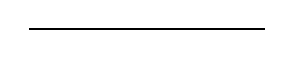
\begin{tikzpicture}[line width=1pt]
    % eckige Spitzen
    % benoetigt \usetikzlibrary{arrows}
    \draw[[-{]}] (0, 0) -- (3, 0);
  \end{tikzpicture}
\end{minipage}

\begin{minipage}{0.7\textwidth}
  \footnotesize
  % parcolor version 2011-09-30
\begingroup
\ttfamily
\definecolor{R}{named}{Red}
\definecolor{G}{named}{ForestGreen}
\definecolor{B}{named}{RoyalBlue}
\definecolor{C}{named}{Cyan}
\definecolor{M}{named}{Magenta}
\definecolor{Y}{named}{YellowOrange}
\definecolor{background}{rgb}{0.82, 0.82, 0.92}
\dimen255=\textwidth
\advance\dimen255 by -2\fboxsep
\noindent
\colorbox{background}
{%
\parbox{\dimen255}
{%
\rule[-0.5ex]{0pt}{2.5ex}\hspace*{0.0em}\textcolor{G}{\textbf{\%~benoetigt~\textbackslash{}usetikzlibrary\{arrows\}}}\\
\rule[-0.5ex]{0pt}{2.5ex}\hspace*{0.0em}\textbackslash{}draw[{<}{-}{>},~\textcolor{R}{\textbf{{>}=diamond}}]~(0,~0)~{-}{-}~(3,~0);}%
}%
\endgroup

\end{minipage}\hfill
\begin{minipage}{0.29\textwidth}
  \centering
  \begin{tikzpicture}[line width=1pt]
    % Form: diamond
    % benoetigt \usetikzlibrary{arrows}
    \draw[<->, >=diamond] (0, 0) -- (3, 0);
  \end{tikzpicture}
\end{minipage}

